
\section{História e Narrativa}

O mago Ogof, sedento por poder, capturou três seres místicos, em três diferentes épocas para o seu ritual ardiloso. Quando os planetas se alinham ele captura o gato de uma bruxa, a esposa de um elfo e o filho de um xamã. O ritual espalhou pelo mundo 3 joias que guardam as almas dos raptados. Resgate as joias com esses três personagens jogáveis, mas o ritual só é reversível com as três joias juntas.

\section{Áreas do Jogo}

\subsection{O mundo de Ogof}
Mesopotâmia, idade antiga. Ogof vive na cidade de Ur na época de 4000 a.C. à 1900 a.C. Uma sociedade hidráulica onde todo o estilo de vida gira em torno de seus rios Tigre e Eufrates. Para tal, desenvolveram grandes habilidades arquitetônicas para lidar com as enchentes .

A sociedade residente de Ur é estamental, isto é, pessoas nascidas em uma determinada classe social morrerão nessa mesma classe e sua política tem bases religiosas. Isso significa que um líder político é necessariamente alguém que se diz parente ou conhecido de algum deus.

\subsection{O mundo dos Duendes}
Baseada em Geiranger, Noruega - 1920
Situado em um belo fiorde, suas terras são afastadas dos outros lugares pelas montanhas rochosas que a cercam, e a forma mais fácil de chegar a essas terras é por um navegante que tenha habilidade suficiente para navegar pelo mar através dos
fiordes, o que não é tarefa fácil. Por essa razão duendes são seres desconhecidos e ocultos que transitam com facilidade pelo mundo dos humanos e os ajudam se julgarem que tem boa índole, do contrário podem atrapalhar muito suas vidas escondendo coisas, assustando animais e fazendo ruídos assustadores. Em ambos os casos duendes nunca devem ser vistos.

Algumas histórias de ninar como o "Conto do Sapateiro" narram a história de humanos que descobriram os duendes e, cheios de gratidão, lhe presentearam com roupas e assistiram satisfeitos a sua partida acreditando que os duendes haviam encerrado o seu trabalho e partiram felizes. Mas, para a sociedade destes seres misticos a regra é clara: receber roupas significa que você foi descoberto e desonrou as tradições do seu povo, a sentença é o banimento.

\subsection{O mundo da Bruxa}
\subsection{O mundo do Xamã}
Baseado na antiga aldeia indígena Mesa Verde, nos Estados Unidos que data de 1400 anos atrás, tendo existido por cerca de 700 anos. Os índios dessa aldeia tinham características como:


\section{Personagens}
\subsection{Ogof}
\textbf{Back history: }Sedento por conhecimento, acessou ensinamentos ocultos que desestabilizaram sua mente e agora o poder é sua obsessão.

\textbf{Físico:} velho, parrudo, imponente. Com uma barba longa e grisalha.

\textbf{Descrição psicológica:} Impiedoso e insano, ocasionalmente fala coisas sem sentido.

\textbf{Arquétipo:} Sombra

\subsection{Duende}
\textbf{Back history:} Trabalhador com uma rotina tediosa e repetitiva. Seu mal humor é apenas curado por sua esposa doce.

\textbf{Descrição física:} Pequeno, gordo e mal vestido.

\textbf{Descrição psicológica:} Temperamental, revoltado e mau humorado.

\textbf{Arquétipo:} Pícaro

\textbf{Temperamento:} Irritadiço quando está com o contador de vida cheio. Quando o contador está próximo do fim fica furioso.

\textbf{Iteração: } Neste universo, duendes são seres misticos que coexistem com humanos. Parte dos desafios é manter-se despercebido. São mais facilmente vistos por crianças.

\textbf{Habilidades: }
\begin{itemize}
\item  Invisibilidade: Auxilia na furtividade do personagem mas depende diretamente dos recursos que o jogador possui. Ao longo da fase deverá coletar maçãs que encherão uma barra de energia que, quando completa, libera a invisibilidade. O jogador deve gerenciar a barra para usá-la em obstáculos estratégicos.
\end{itemize}


\begin{itemize}
\item Chuva:  funciona da mesma forma que a invisibilidade, ao coletar uma quantidade de bananas suficiente para encher a barra poderá invocar chuva, mas deverá administrar os recursos com cautela.
\end{itemize}
Ambos os itens, maçãs e bananas são adquiridos tanto buscando-os em esconderijos no cenário quanto prestando favores aos humanos.

\textbf{Fraqueza:} De acordo com [N˜AO LEMBRO QUEM DISSE ISSO] duendes são seres desatentos e facilmente distraíveis. Para simular essa característica, o jogador só pode enxergar com clareza poucos metros de distância a partir do duende. Ao restante do cenário foi adicionado um desfoque para que seja levemente borrado, dificultando a identificação dos elementos.

\subsection{Bruxa}

\begin{figure}[htb]
	\caption{concept Bruxa}
	\begin{center}
	    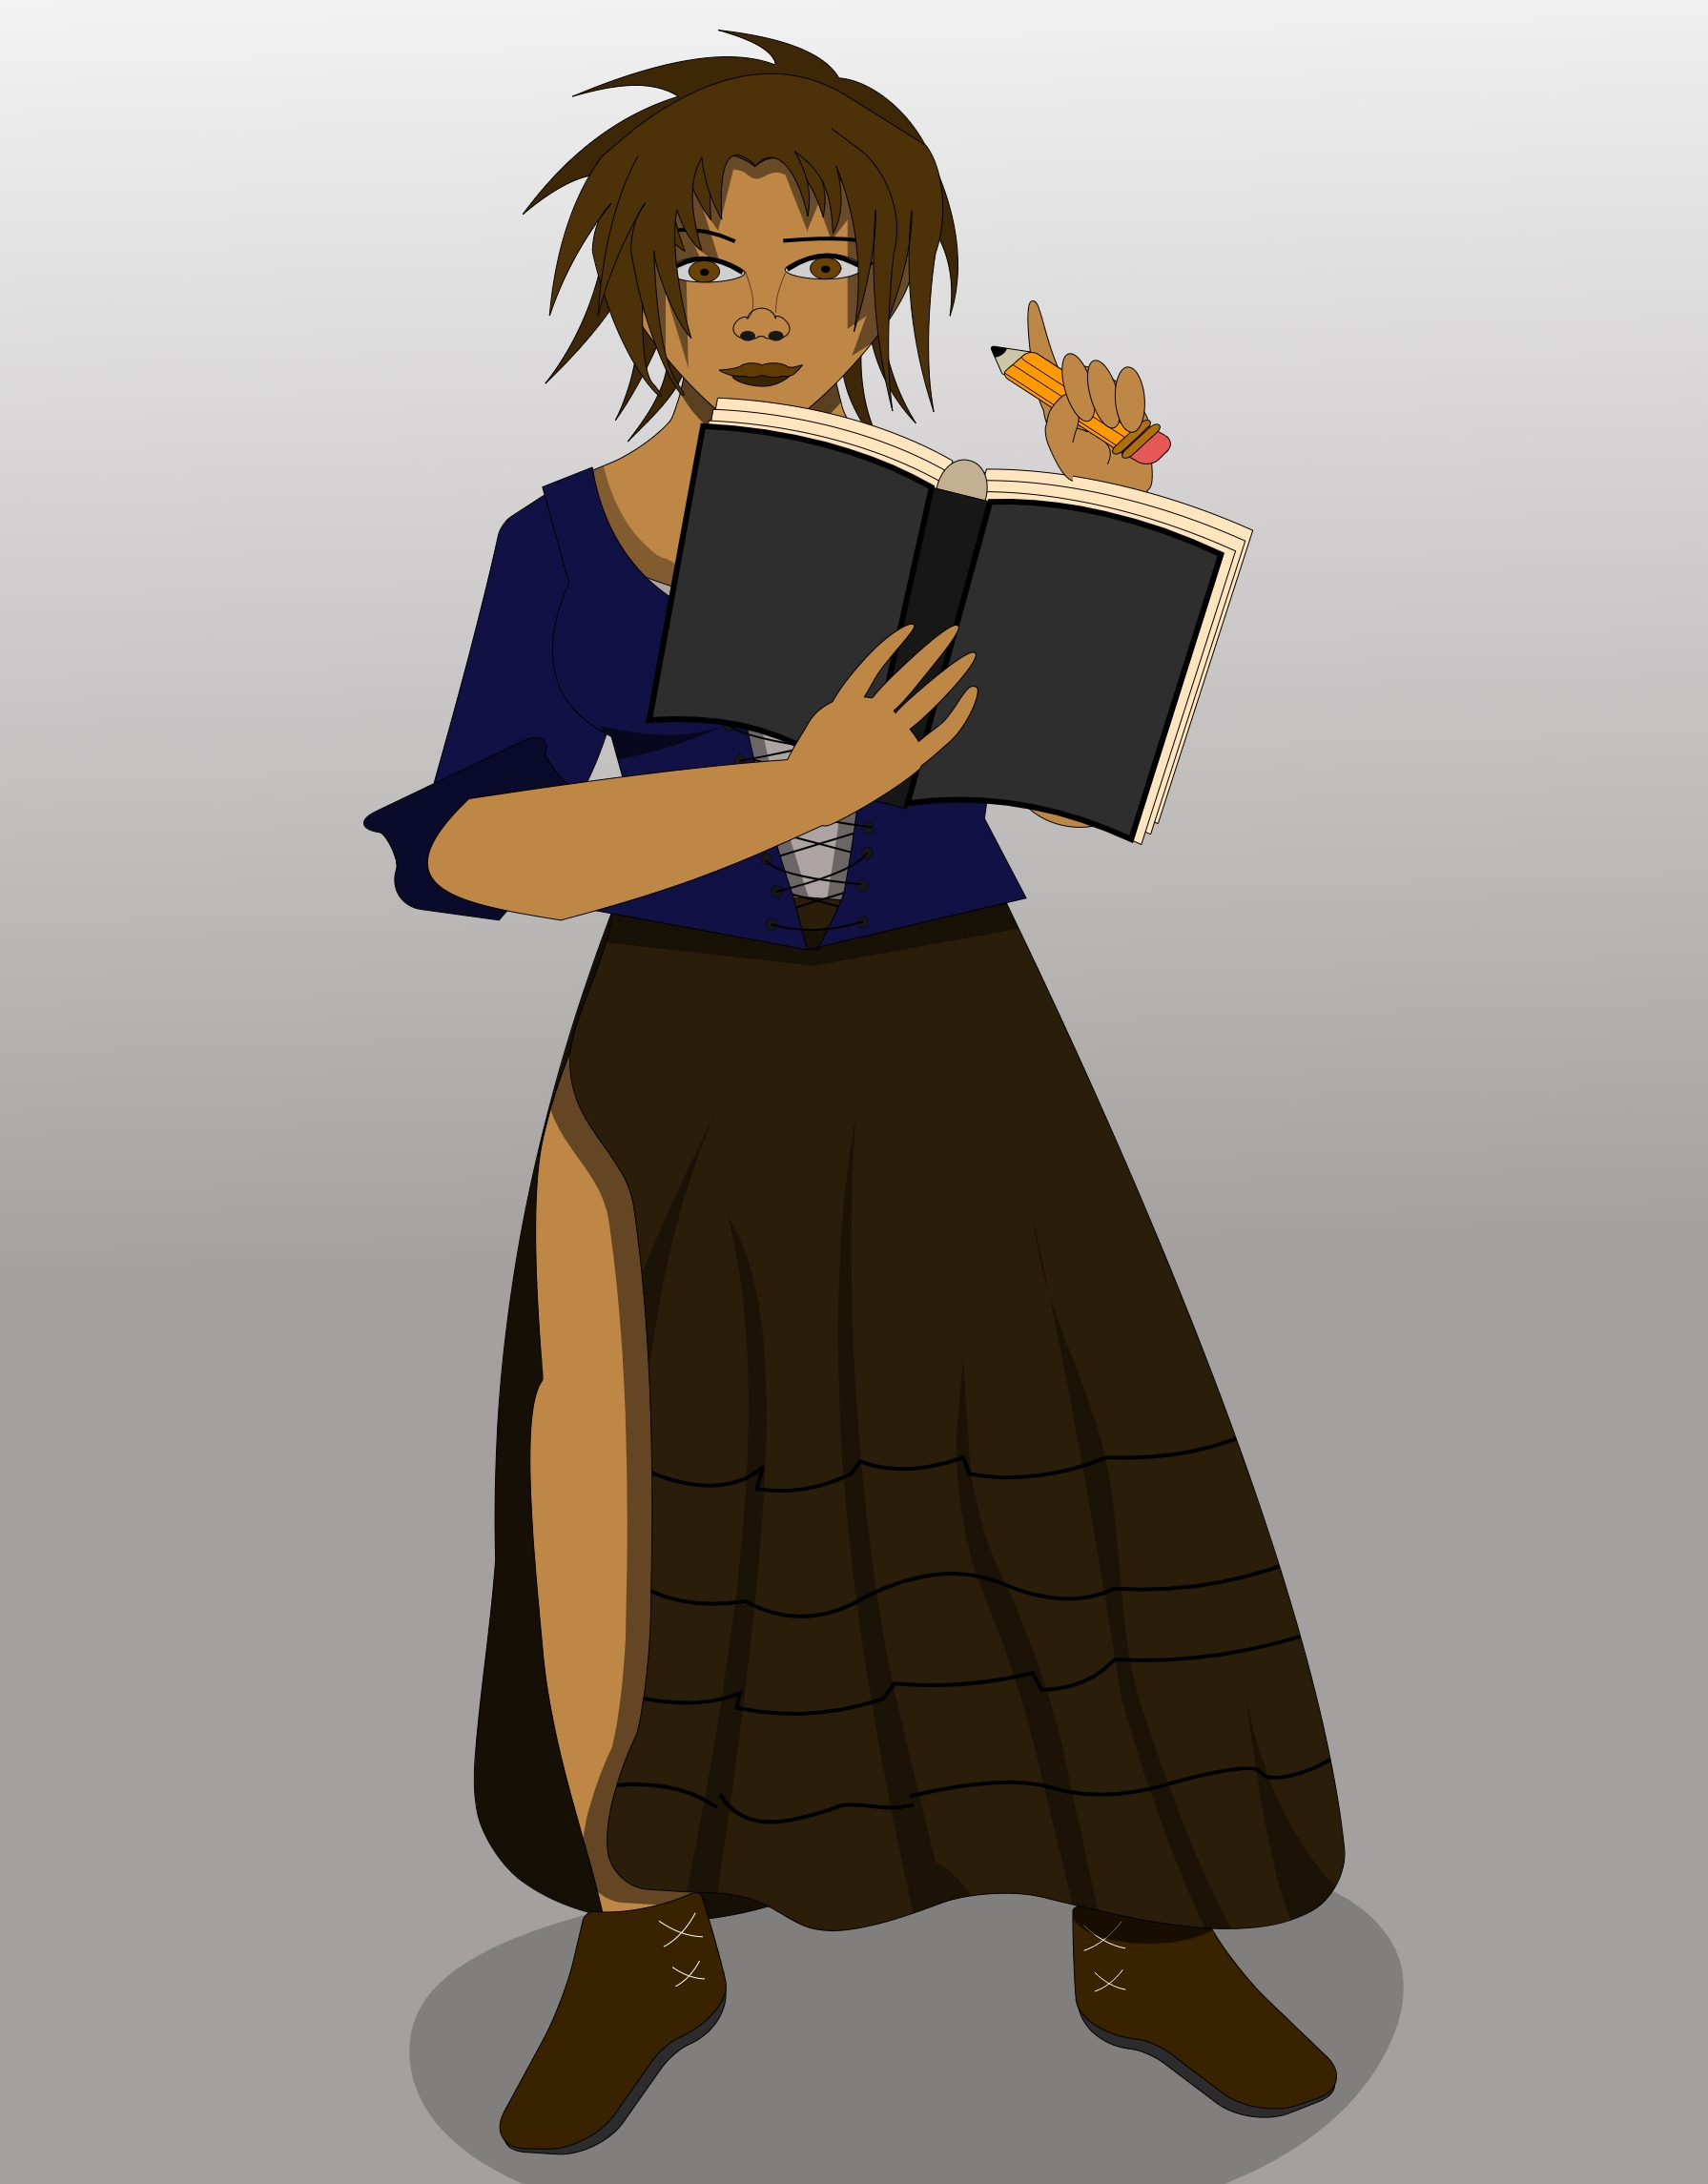
\includegraphics[width=\textwidth/2]{imagens/capaportifolio.jpeg}
	\end{center}
	\legend{Fonte: Própria Autoria(Marina Araujo)}
\end{figure}


\textbf{Back history:} Estudiosa e conhecedora das artes do oculto. Respeita as artes mágicas e não faz uso sem autorização. Treinada pelas anciãs.

\textbf{Descrição física/psicológica:} Metamorfa, sua personalidade é afetada pela energia do ambiente. Quando suas energias são boas e prestativas assume a aparência de bruxa má. Quando a escuridão a consome se torna uma mulher bela e jovem.

\textbf{Arquétipo: }Camaleão

\subsection{Xamã}

\textbf{Back history: }indígena norte americano, sábio e orientador da tribo.

\textbf{Descrição física: }Pele vermelha, e aparência respeitável. Inspira confiança mas intimida. Utiliza pele de lobo na cabeça.

\textbf{Descrição psicológica:} Sério e protetor como um grande pai. Transcende o corpo e trabalha com espíritos para proteger o grupo.

\textbf{Arquétipo:} Mentor

\section{Fases}

\subsection{A Redenção de um duende -- Fullkomnun}
O duende chega a tempo de ver Ogof levando sua esposa e o persegue até conseguir arrancar-lhe um pedaço da roupa, mas não consegue impedi-lo. O mestre da vila se aproxima e encontra o duende enfurecido. Percebendo que ele tem uma pedaço de roupa nas mãos,  manda que encontre o ancião a procura de ajuda.
O ancião então lhe diz que, para abrir o portal pelo qual Ogof fugiu serão necessários itens humanos [A DEFINIR] e itens de agricultura. O duende então sai em busca destes itens.

\subsubsection{O pico do fiorde}
O  ancião vive no ponto mais alto do reino: o topo de um icônico fiorde. Sob o ar rarefeito e a densidade da nevoa, apenas os duendes mais resistentes e determinados conseguem chegar a sua morada e assim receber como recompensa as suas sábias orientações.

\subsubsection{A plantação de Elvdans}
A cidade de Elvdans é povoada por camponeses humanos, um povo simples e supersticioso, porém amigável. O jogador deverá encontrar uma plantação suntuosa na cidade, onde uma família de duendes deixara itens mágicos para trazer prosperidade. Os fazendeiros não necessitam mais delas, você deve levá-las consigo para atender a ordem do ancião e posteriormente deixa-los a vista para que outro humano os pegue. Duendes são uma especie temperamental e emotiva por isso tem tendências a ajudar pessoas ao longo de suas viagens. Quando o usuário interromper seus afazeres para auxiliar alguém receberá itens que lhe serão uteis mais tarde.

\subsection{O Lobo Guardião}

O Xamã meditava concentrado quando um índio interrompe seu momento mais intimo para avisar que algo acontecera com seu filho. O protagonista corre para a sua casa e a encontra revirada e vazia.

No topo do cânion onde vivem os aldeões, existe uma águia mística que serve ao Xamã. Ela o ajudará a encontrar Ogof.

\subsubsection{O topo do cânion}
Saindo da casa do Xamã, o jogador deve seguir por tuneis obscuros para chegar ao topo do cânion onde encontrará a águia. Conectando-se com o animal o personagem será capaz de ver através de seus olhos. A ave sobrevoa os arredores mostrando rastros do caminho de Ogof até uma passagem onde um portal fora aberto.

\subsubsection{O Mercado}
Com as informações concedidas pela águia, o Xamã deve agora voltar pelos túneis e seguir até o mercado local que consiste em uma pequena feira ao ar livre de onde pode-se comprar os itens necessários para reabrir o portal.

O personagem deve coletar itens ao longo do caminho para forjar um arco e flecha que servirá como moeda de troca para a mercadoria.

\subsubsection{Portal}
Seguindo todos os rastros de Ogof, o Xamã chega até o outro lado do cânion. Adentra uma passagem e alinha os itens que comprou no mercado em cima de um pedestal, uma passagem outrora oculta se abre.

\section{Fase de Treino e/ou Tutorial}

O treino de habilidades será feito de forma imersiva para o jogador, nas fases em que ele jogará com apenas um personagem, sendo elas apresentadas de forma gradual ao jogador.
